\documentclass[a4paper,10pt]{article}
\usepackage[english]{babel}
\usepackage[utf8]{inputenc}
\usepackage{graphicx}
\usepackage{amsmath,amssymb}
\usepackage{hyperref, url}
\usepackage{listings}
\usepackage[multiple]{footmisc}
\usepackage[english]{babel}
\usepackage{float}
\parindent 0mm
\parskip 3mm

% add your name and student number in parenthesis
\title{ICS-E4020: Week 6 - Challenge}
\author{Néstor Castillo García (472081)\\ 
       {\tt nestor.castillogarcia@aalto.fi}}
\begin{document}

\maketitle

\section{Challenge Submissions}

\subsection{Description}

The previous implementations were compared and results are shown in the same report. No extra assignments were implemented.

\subsection{Hardware}
The computers had the following specifications: Intel Xeon E3-1230v2, 4 cores, 8 thread, 3,3 GHz, RAM: 16 GB, GPU: Nvidia K2000.


\subsection{Median Filter}
A median filter was implmented for png images such that for each colour component, the value of each pixel is the median of all pixel values within a sliding window of dimensions (2k+1) x (2k+1).

An eight threaded solution solves the median filtering in an image in less than a quarter of the time of a single threaded solution. It is not an eight due to the fact that only four threads with hyperthreading are being used. The complexity of the median function is O(n). This implementation could be improved to minimise memory access and execute many calculation with minimum data read.

\begin{figure}[H]
\centering
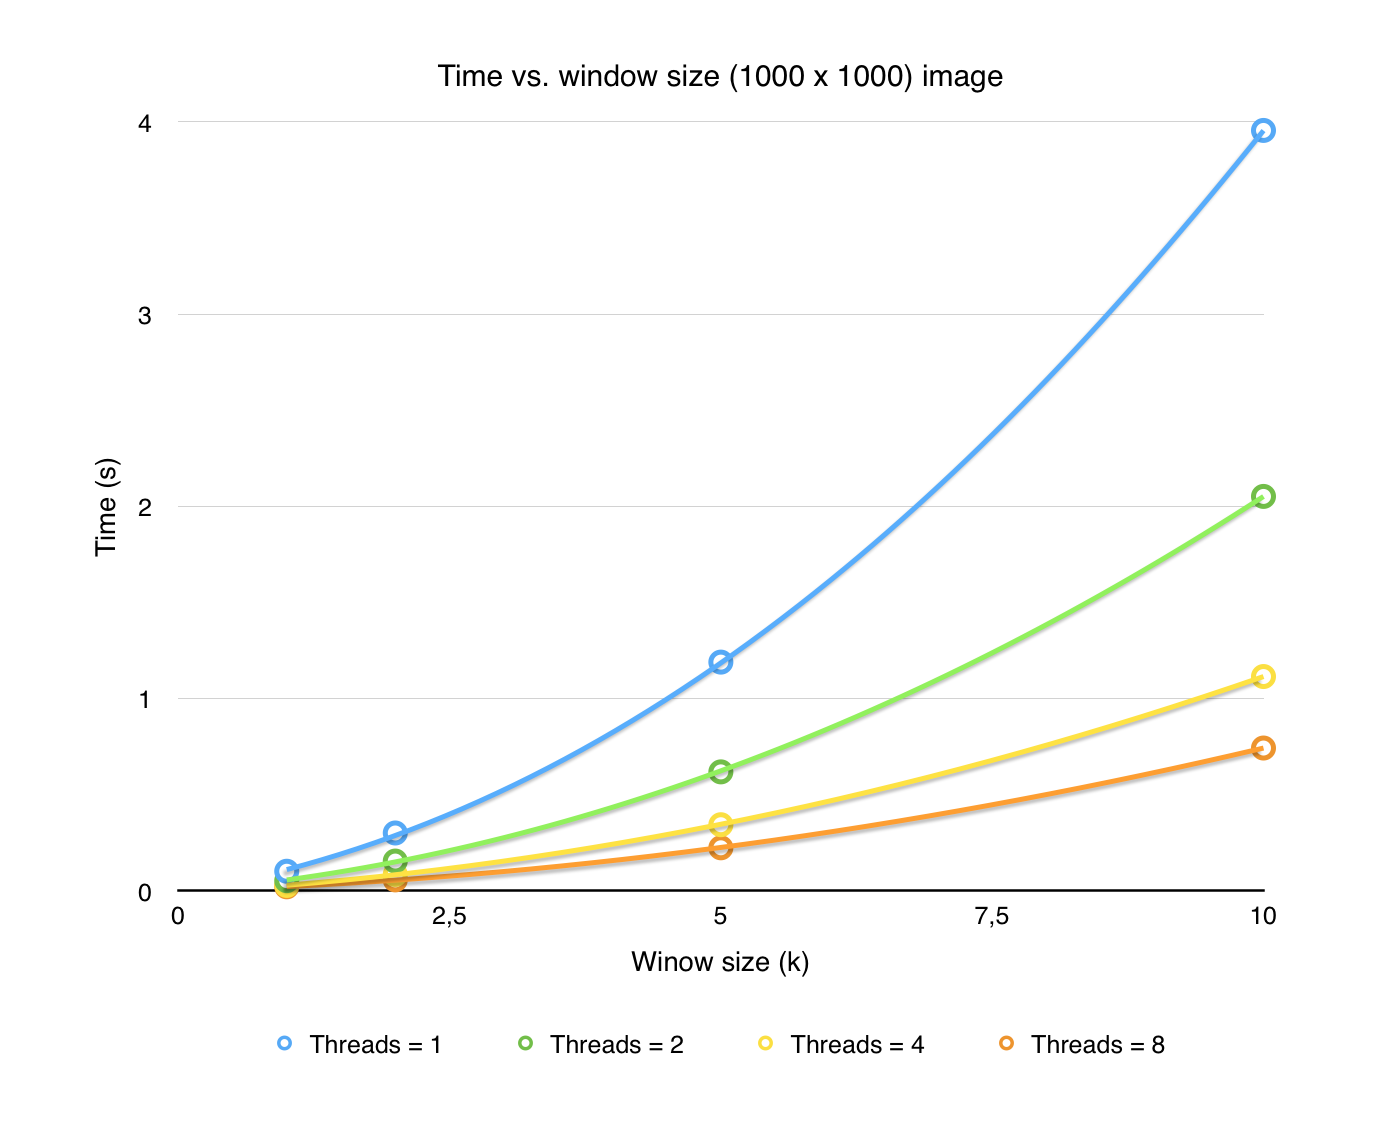
\includegraphics[width=1\textwidth]{figures/w1_timeVsSize}
\caption{Meedian filtering window sizes time execution with different number of threads}
\label{fig:pca_type}
\end{figure}

\subsection{Correlated Pairs}
In this task, m input vectors with n numbers are given. The correlations between all pairs of input vectors is calculated. A red pixel at (i, j) indicates a positive correlation between vectos i and j, and a blue pixel indicates a negative correlation. 

The GPU version did the correlated pairs task of a 4000 x 4000 image in less than 1s; 10 times faster than a eight-threaded. The focus of this approach was to maximise the number of arithmetic operation per memory transfer and also to used shared memory per block of threads because it is much more faster than the global memory. 

In the CPU the use of vector registers is extremely useful to increase speed of arithmetic operations.

\begin{figure}[H]
\centering
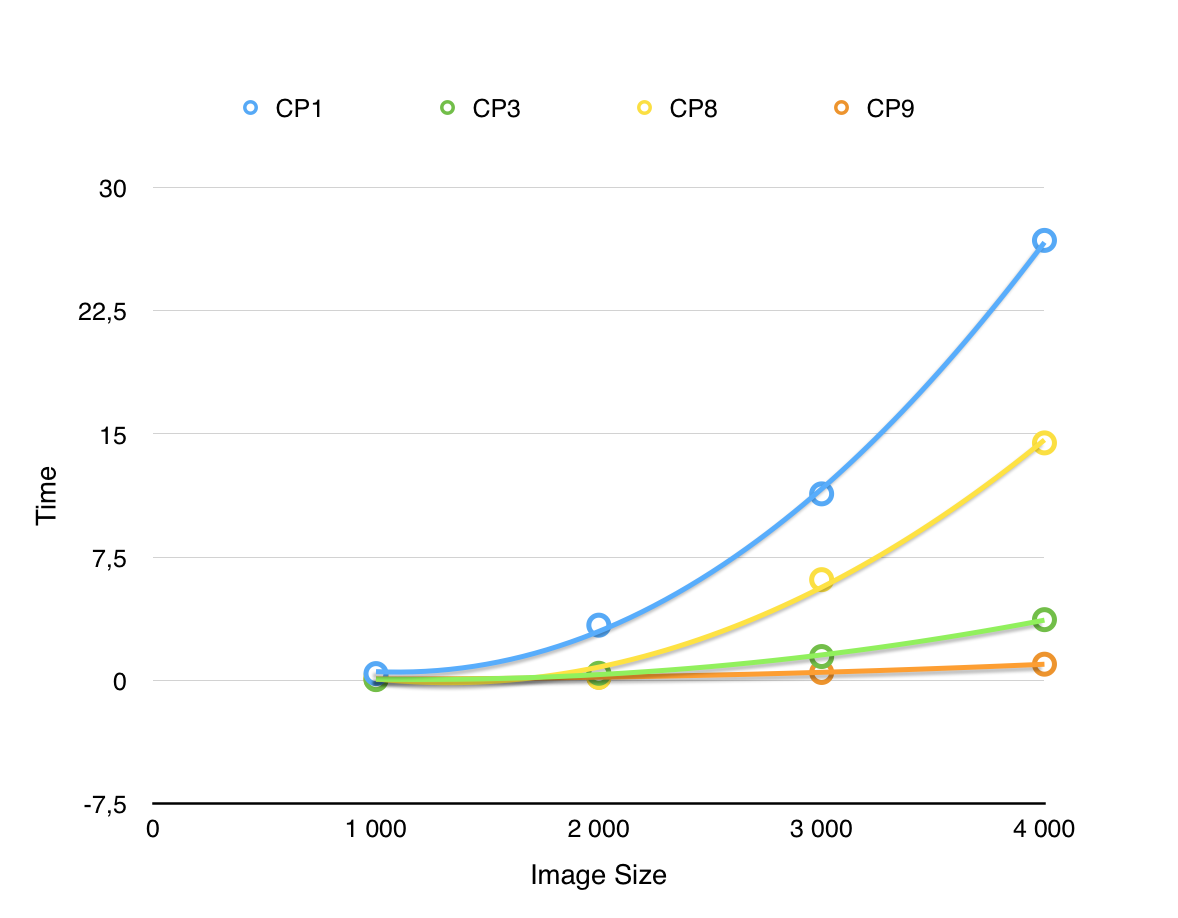
\includegraphics[width=1\textwidth]{figures/w5-comparison}
\caption{Scalability comparison between single threaded, multithreaded, multithreades vectorized and GPU implementations}
\label{fig:pca_type}
\end{figure}

The block size should be a careful selection and if shared mamory is used, the memory per block must be calculated to ensure a correct paralel execution according to the hardware. 

\begin{figure}[H]
\centering
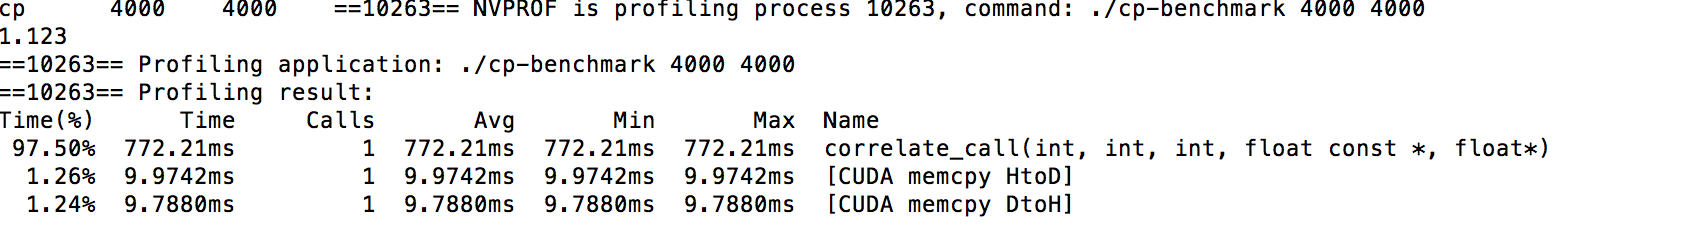
\includegraphics[width=1.3\textwidth]{figures/w5_timing}
\caption{Detailed execution time in a 4000 x 4000 image in comparison to cp8 in cp9 memcopy appears to be a more relevant due to the increased efficiency in arithmetic intensity}
\label{fig:pca_type}
\end{figure}

\begin{figure}[H]
\centering
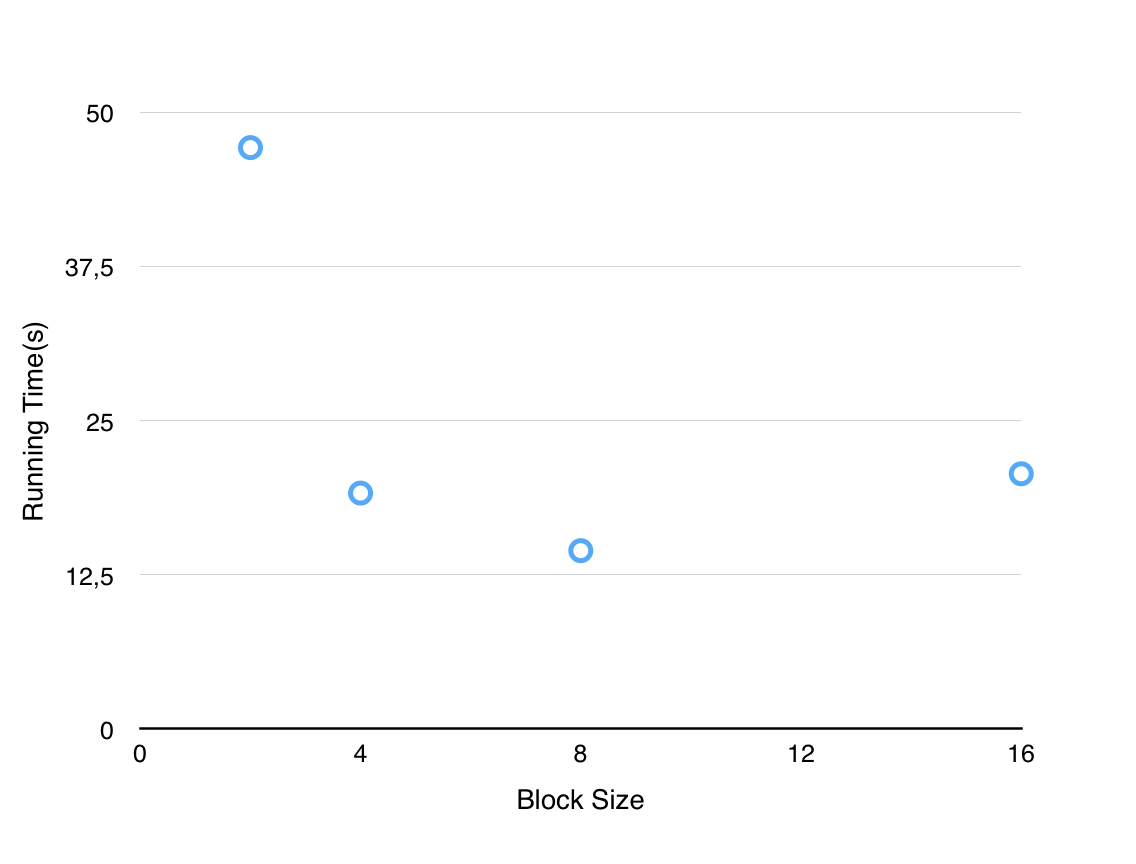
\includegraphics[width=1\textwidth]{figures/w4_timevsBlockSize}
\caption{Time vs BlockSize (squared) in a 4000 x 4000 image}
\label{fig:pca_type}
\end{figure}


\subsection{Sorting}
In this task a parallel version of merge sort was implemented. In the first step the data is divided into n parts and each thread sorts a single part. Then the parts are merged in parallel by pairs until a single sorted chunk is obtained. The algorithm performs better if the number of threads is a power of two.

As expected, performance increased with the number of threads. The multithreded version was in average 3,8 times faster than the single threaded solution for the large random case values. In the other cases there was a slight increase in speed.

\begin{figure}[H]
\centering
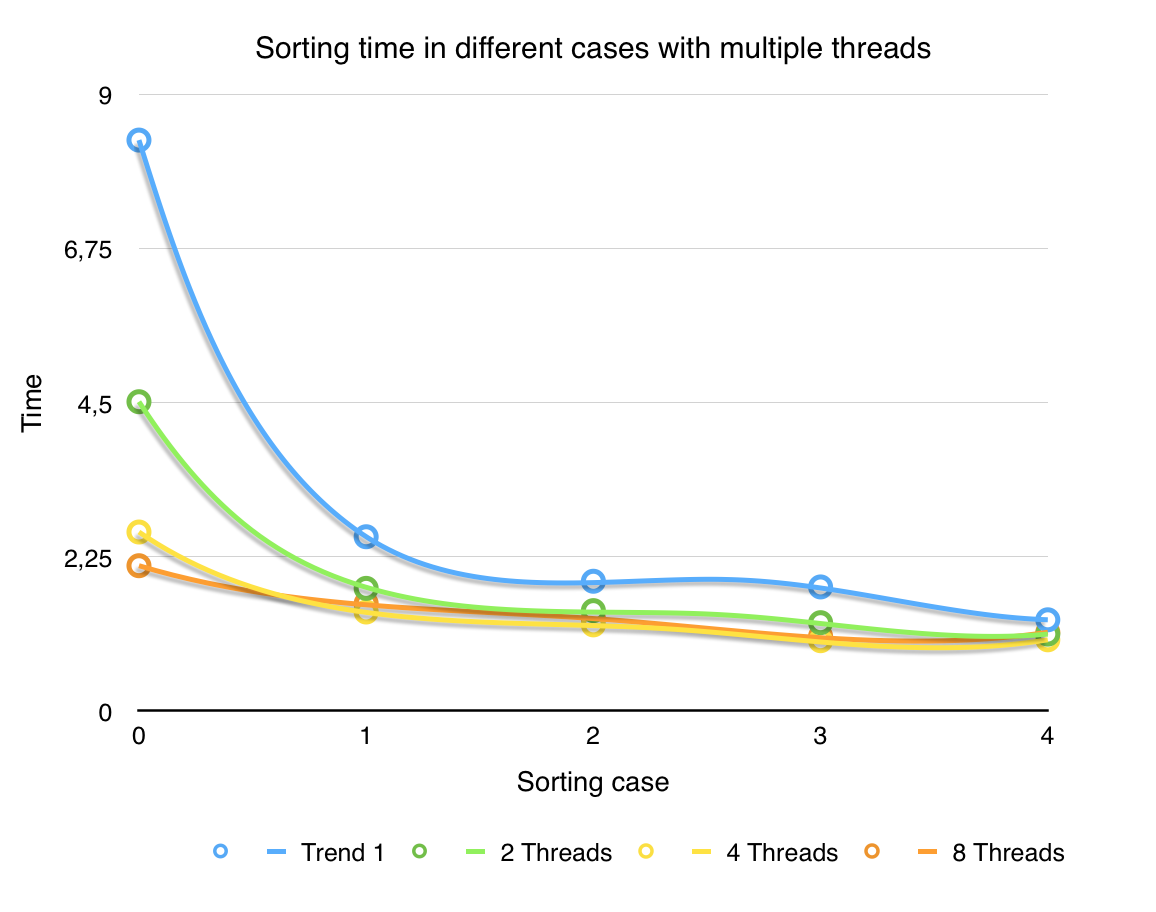
\includegraphics[width=1\textwidth]{figures/w3_SortingTime}
\caption{Multithreaded sorting time in cases:  0 = large random elements, 1 = small random elements, 2 = constant input, 3 = increasing values, and 4 = decreasing values.}
\label{fig:pca_type}
\end{figure}

\subsection{Tables}

The following table contains the benchmark results for different image sizes and number of threads in median filter. 

\begin{table}[h]
\begin{tabular}{|l|l|l|l|l|l|l|}
\hline
\textbf{img. width} & \textbf{img. height} & \textbf{k} & \textbf{Threads = 1} & \textbf{Threads = 2} & \textbf{Threads = 4} & \textbf{Threads = 8} \\ \hline
100                 & 100                  & 1          & 0,003                & 0,001                & 0,001                & 0,001                \\ \hline
100                 & 100                  & 2          & 0,007                & 0,002                & 0,002                & 0,002                \\ \hline
100                 & 100                  & 5          & 0,023                & 0,006                & 0,004                & 0,006                \\ \hline
100                 & 100                  & 10         & 0,038                & 0,02                 & 0,013                & 0,017                \\ \hline
200                 & 200                  & 1          & 0,004                & 0,002                & 0,002                & 0,001                \\ \hline
200                 & 200                  & 2          & 0,012                & 0,007                & 0,006                & 0,003                \\ \hline
200                 & 200                  & 5          & 0,048                & 0,026                & 0,016                & 0,011                \\ \hline
200                 & 200                  & 10         & 0,156                & 0,081                & 0,044                & 0,03                 \\ \hline
500                 & 500                  & 1          & 0,025                & 0,013                & 0,01                 & 0,006                \\ \hline
500                 & 500                  & 2          & 0,075                & 0,039                & 0,028                & 0,017                \\ \hline
500                 & 500                  & 5          & 0,297                & 0,155                & 0,088                & 0,057                \\ \hline
500                 & 500                  & 10         & 0,986                & 0,511                & 0,277                & 0,187                \\ \hline
1000                & 1000                 & 1          & 0,102                & 0,053                & 0,028                & 0,021                \\ \hline
1000                & 1000                 & 2          & 0,301                & 0,155                & 0,085                & 0,057                \\ \hline
1000                & 1000                 & 5          & 1,19                 & 0,619                & 0,344                & 0,224                \\ \hline
1000                & 1000                 & 10         & 3,956                & 2,052                & 1,115                & 0,743                \\ \hline
2000                & 2000                 & 1          & 0,407                & 0,212                & 0,133                & 0,08                 \\ \hline
2000                & 2000                 & 2          & 1,198                & 0,621                & 0,328                & 0,226                \\ \hline
2000                & 2000                 & 5          & 4,764                & 2,479                & 1,336                & 0,898                \\ \hline
2000                & 2000                 & 10         & 15,867               & 8,229                & 4,346                & 2,982                \\ \hline
\end{tabular}
\end{table}



\begin{figure}[H]
\centering
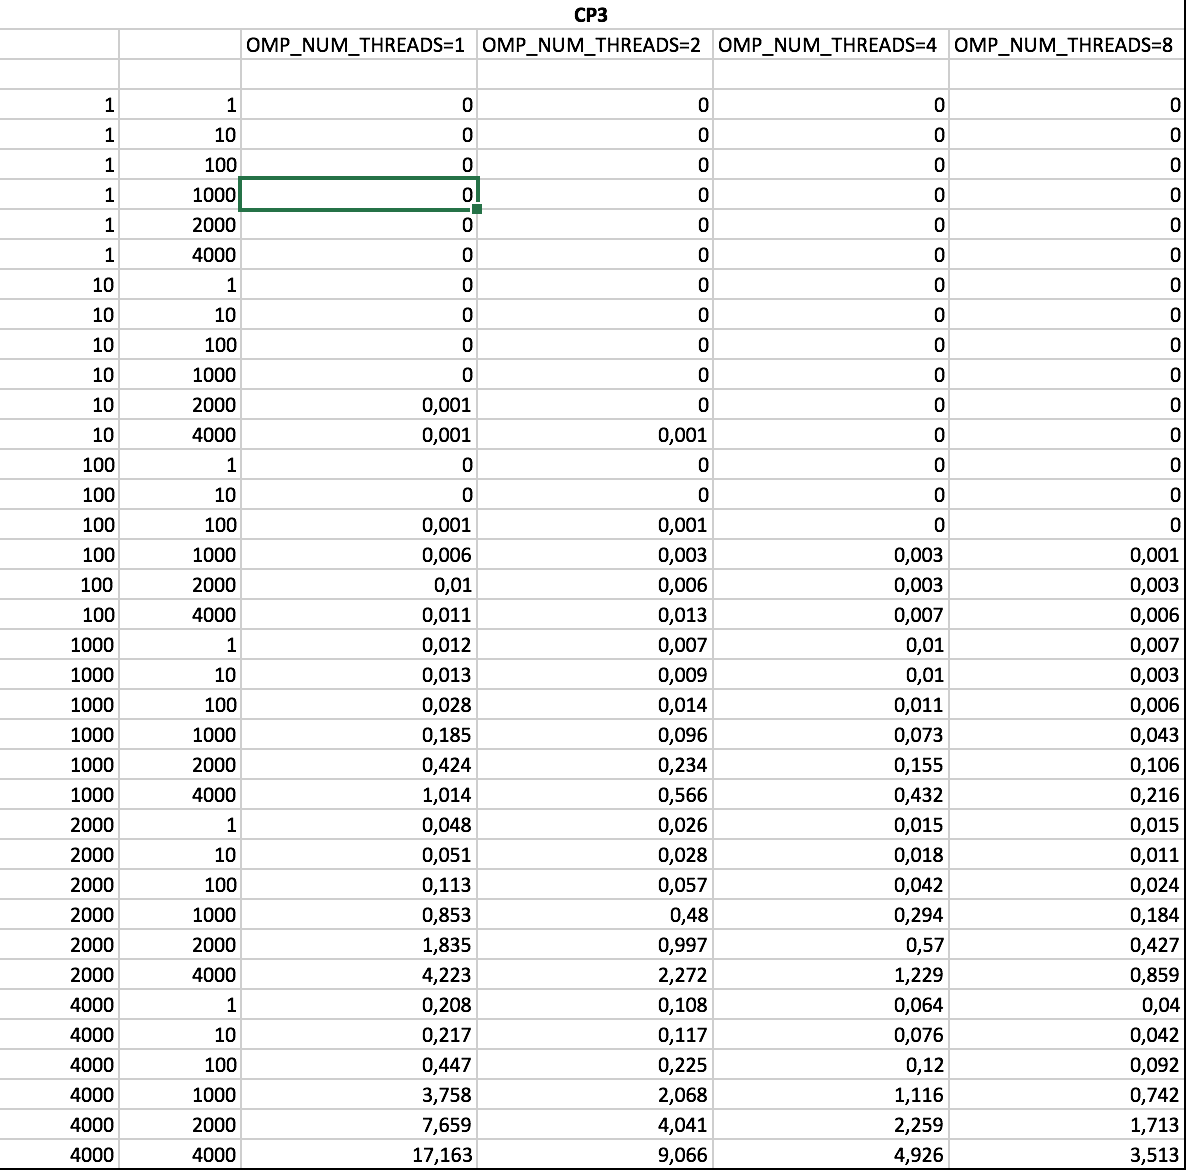
\includegraphics[width=1\textwidth]{figures/w2_cp3}
\caption{CP3 benchmark result with different number of cores}
\label{fig:pca_type}
\end{figure}

\begin{figure}[H]
\centering
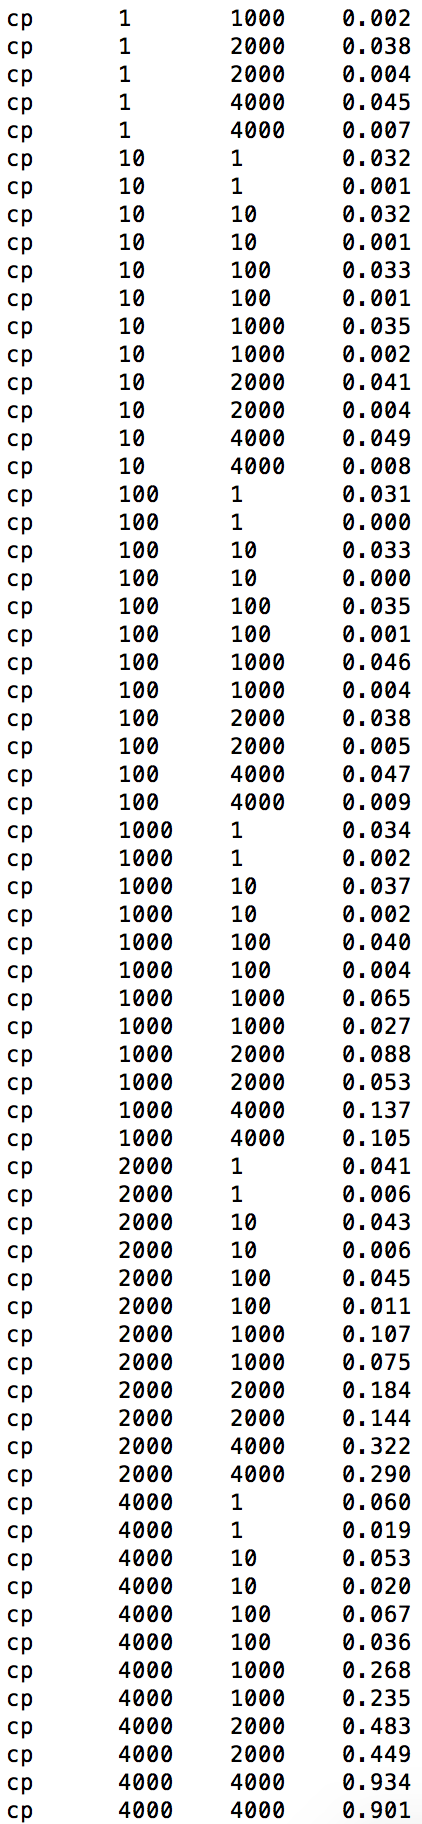
\includegraphics[width=0.3\textwidth]{figures/w5_benchmark}
\caption{Benchmark results for GPU correlated pairs implementation CP9}
\label{fig:pca_type}
\end{figure}







I\end{document}